\documentclass[12pt, a4paper]{article}
\usepackage{bm, float,amsmath,graphicx}
\graphicspath{ {./images/} }
\usepackage[T1]{fontenc}
\usepackage[polish]{babel}
\usepackage[utf8]{inputenc}

\title{Opracowanie zadania z geometrii obliczeniowej}
\author{Stepan Yurtsiv, 246437}

\begin{document}
\maketitle

\section*{Definicje}

\subsubsection*{Wielokąt prosty}

Wielokąt prosty to taki wielokąt, którego boki się nie przecinają oraz tworzą jedną zamkniętą łamaną (patrz rysunek \ref{fig:wielokat_prosty} i \ref{fig:wielokat_nieprosty}).

\begin{figure}[H]
  \begin{center}
  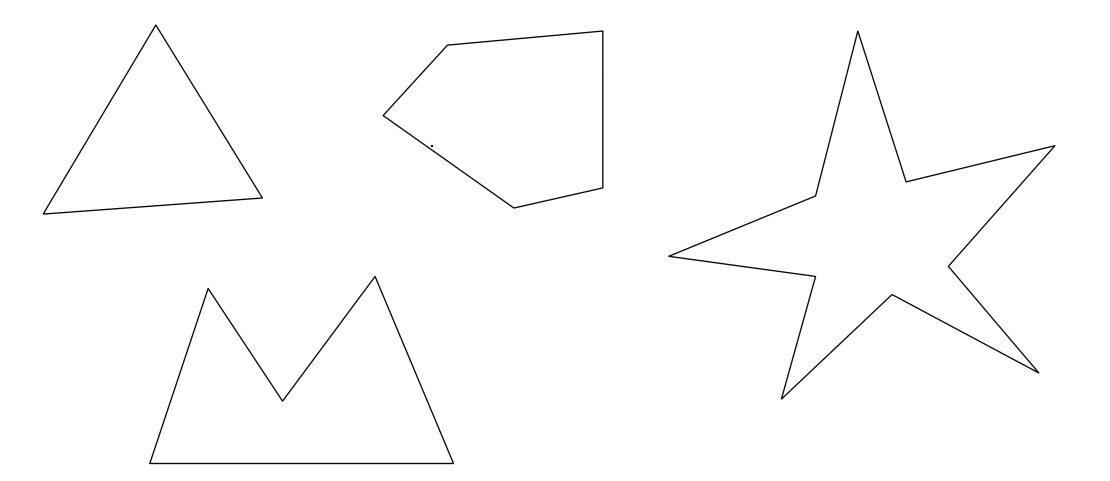
\includegraphics[scale=0.4]{Prosty}
  \caption{Przykłady wielokątów prostych}
  \label{fig:wielokat_prosty}
  \end{center}
\end{figure}

\begin{figure}[H]
  \begin{center}
  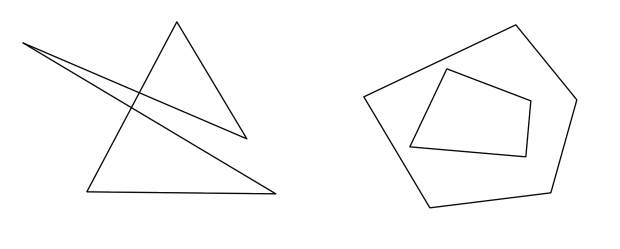
\includegraphics[scale=0.5]{Nieprosty}
  \caption{Przykłady wielokątów nieprostych}
  \label{fig:wielokat_nieprosty}
  \end{center}
\end{figure}

\subsubsection*{Wielokąt monotoniczny}

Wielokąt monotoniczny to taki wielokąt, dla którego możemy podać prostą $L$, taką że każda prosta prostopadła do niej przecina wielokąt w najwyżej dwóch punktach (silna monotoniczność). Słabą monotonicznością nazywamy przypadek, gdy wielokąt posiada również krawędzie
prostopadłe do $L$. Na rysunku \ref{fig:wielokat_monotoniczny} dwa górne wielokąty są monotoniczne. Zielone proste mają jedno przecięcie z wielokątem, niebieskie – dwa, czerwone – trzy i więcej.

\begin{figure}[H]
  \begin{center}
  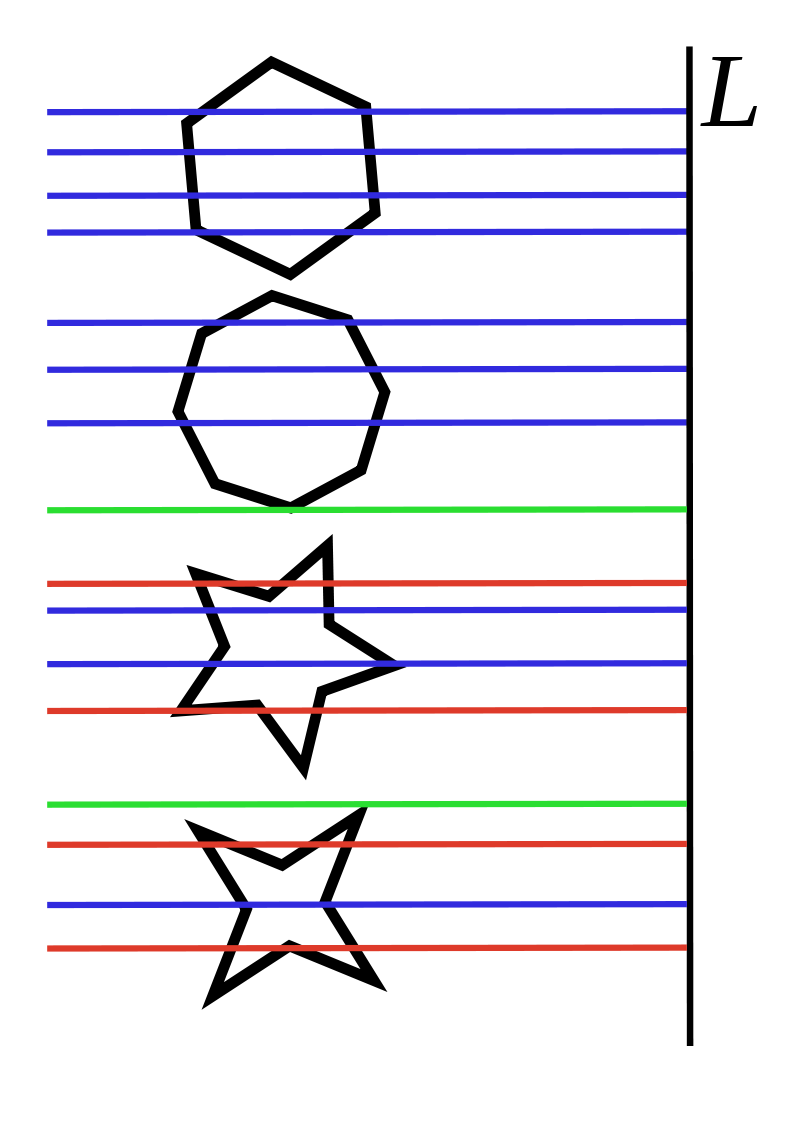
\includegraphics[scale=0.3]{Monotonic}
  \caption{Monotoniczność wielokątów (źródło: Wikipedia)}
  \label{fig:wielokat_monotoniczny}
  \end{center}
\end{figure}


\section*{Zadanie}

Podaj efektywny alogrytm do sprawdzenia czy dany $n$ kąt prosty jest monotoniczy względem podanej prostej (zadanie 10 na liście).
 
\section*{Algorytm}

Rozważmy instację problemu, przedstawioną na rysunku 

\begin{figure}[H]
  \begin{center}
  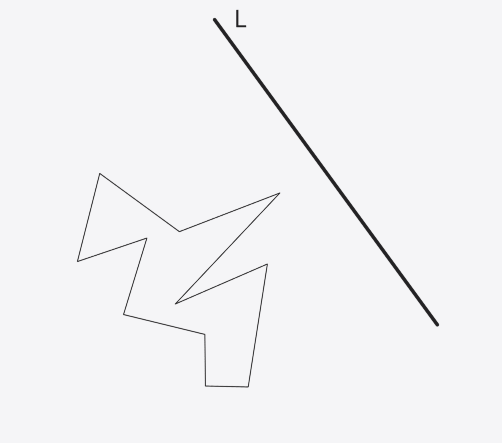
\includegraphics[scale=0.3]{Sample1}
  \caption{Monotoniczność wielokątów (źródło: Wikipedia)}
  \label{fig:instancja_1}
  \end{center}
\end{figure}

\end{document}
